% SwegHammer project handout — intended for printing and handing out to
% people unfamiliar with both Warhammer 40K and this project.
% Build: pdflatex HANDOUT.tex  (run twice for ToC / cross-refs)

\documentclass[11pt,a4paper]{article}

\usepackage[T1]{fontenc}
\usepackage{lmodern}
\usepackage[margin=25mm]{geometry}
\usepackage{xcolor}
\usepackage{hyperref}
\usepackage{booktabs}
\usepackage{array}
\usepackage{tabularx}
\usepackage{graphicx}
\usepackage{enumitem}
\usepackage{amsmath}
\usepackage{tikz}
\usetikzlibrary{arrows.meta, positioning}

\definecolor{simblue}{HTML}{1F6FB2}
\definecolor{realorange}{HTML}{D2691E}
\definecolor{greentick}{HTML}{2E8B57}
\definecolor{greytext}{HTML}{555555}

\hypersetup{
  colorlinks=true,
  linkcolor=simblue,
  urlcolor=simblue,
}

\setlength{\parindent}{0pt}
\setlength{\parskip}{6pt}

% Compact section headers
\usepackage{titlesec}
\titleformat{\section}{\Large\bfseries\color{simblue}}{}{0em}{}
\titleformat{\subsection}{\large\bfseries\color{greytext}}{}{0em}{}

\newcommand{\statbox}[2]{\textbf{#1}\,#2}

\begin{document}

% ── Title ──────────────────────────────────────────────────────────────
\begin{center}
  {\Huge\bfseries\color{simblue} SwegHammer}\\[6pt]
  {\large\itshape A simulation-driven approach to balancing Warhammer 40,000}\\[4pt]
  {\small\color{greytext} Project handout — June 2026}
\end{center}

\vspace{4mm}
\hrule height 0.8pt
\vspace{6mm}

% ── Section 1: What is Warhammer 40K? ─────────────────────────────────
\section{What is Warhammer 40,000?}

Warhammer 40,000 (often shortened to 40K) is a tabletop miniatures game set
in a far-future science-fiction universe. Two players assemble armies of
detailed plastic miniatures, deploy them on a terrain-covered table, and
fight a battle over five rounds using dice rolls, measuring tapes, and thick
rulebooks.

The game is published by Games Workshop and is currently in its 10th Edition.
If you want a feel for the basic rules, the quick-start guide is freely
available online:

\begin{center}
  \url{https://wahapedia.ru/wh40k10ed/the-rules/quick-start-guide/}
\end{center}

\subsection{Datasheets: a unit's identity card}

Every unit in the game has a \textbf{datasheet} --- a page that lists all of
its stats, weapons, and special abilities. Two example datasheets are
reproduced at the end of this handout (pages~\pageref{sec:datasheets}--\pageref{sec:datasheets-end}).
They illustrate the range of complexity in the game: a basic infantry squad
(\textit{Intercessor Squad}) and a towering war machine (\textit{Knight
Crusader}).

Each model in the game has a core stat line:

\begin{center}
\begin{tabular}{ll}
  \toprule
  \textbf{Stat} & \textbf{What it means} \\
  \midrule
  Movement (M)         & How far the model moves each turn, in inches \\
  Toughness (T)        & How hard the model is to wound \\
  Save (Sv)            & Armour save --- roll this or higher on a d6 to block a hit \\
  Wounds (W)           & Hit points; the model is destroyed when these reach zero \\
  Leadership (Ld)      & Morale; lower is better \\
  Objective Control (OC) & How much weight the model carries when holding an objective \\
  \bottomrule
\end{tabular}
\end{center}

Weapons have their own profiles: number of Attacks, Ballistic Skill (the
roll needed to hit), Strength, Armour Penetration, and Damage.

% ── Section 2: The Balance Problem ─────────────────────────────────────
\section{The balance problem}

Warhammer 40,000 is a grossly complex game, with hundreds of unique models,
special abilities, and strategies. Creating a ``balanced game'' is incredibly
tough. When two opponents play a game, a pre-set points limit is agreed
(usually 2,000 for a tournament). Each model, character, tank, and monster
has an in-game points cost. Players build their army up to that limit, so
points are the currency that is supposed to make unlike things comparable:
five cheap infantry squads should, in theory, put up a fair fight against
one expensive super-heavy walker.

These points costs are set by Games Workshop, who own Warhammer. Sometimes
these costs are massively over- or under-tuned, leading to tournaments where
players ``spam'' the best units. This introduces a lot of ``feel bad moments''
and means older models tend to get shelved to gather dust. Players are often
forced to buy models they do not really want in order to keep up with the
competitive meta.

\textbf{The aim of SwegHammer is to eliminate these feel-bad moments} and
attempt to balance the game with a mathematically and simulation-driven
approach to deriving points costs.

% ── Section 3: How the simulator works ─────────────────────────────────
\section{How the simulator works}

At its core, SwegHammer is a stochastic combat simulator that plays out
thousands of 40K battles automatically and measures which units win, which
lose, and by how much. It implements the full 10th Edition rules:

\begin{itemize}[nosep]
  \item All five combat phases: Command, Movement, Shooting, Charge, Fight
        (plus Battleshock at round end).
  \item Real dice rolls for the complete hit $\to$ wound $\to$ save $\to$
        feel-no-pain chain --- no averaging, so the natural variance of the
        game is preserved.
  \item A 2D map with terrain: line-of-sight checks, cover, ruins, and
        objective markers.
  \item Around 1,500 units from the full 10th Edition catalogue, including
        faction rules, detachments, leader auras, and stratagems.
\end{itemize}

\subsection{Measuring balance}

The simulator runs many thousands of matched battles. If a unit is
correctly costed, it should win roughly 50\% of its games when fielded at
equal points against a representative spread of opponents. A unit that wins
significantly more than 50\% is under-costed (too cheap for what it does); a
unit that wins significantly less is over-costed (too expensive).

By measuring this win rate across the entire catalogue, SwegHammer can
identify which units are too strong, which are too weak, and by how much ---
then adjust their points costs to bring everything closer to an even 50\%.

\subsection{The maths: Lanchester's Square Law}

The theoretical backbone comes from \textbf{Lanchester's Square Law}, a
model from military operations research. In aimed-fire combat (where each
combatant picks a specific target), combat power scales with the
\textit{square} of the number of combatants:

\[
  \alpha \cdot A^2 \;-\; \beta \cdot B^2 \;=\; \text{constant}
\]

where $A$ and $B$ are the surviving unit counts on each side, and $\alpha$
and $\beta$ are per-unit combat effectiveness ratings. Side~A wins when
$\alpha \cdot A_0^2 > \beta \cdot B_0^2$.

This means \textbf{numbers matter more than individual quality} --- doubling
the size of your army quadruples your aggregate combat power. The points
system has to account for this: cheap, numerous units need to be priced so
that their squared-count advantage is paid for.

SwegHammer defines a unit's raw effectiveness as:

\[
  e \;=\; \text{health} \;\times\; \text{damage} \;\times\; \text{hit probability}
\]

and anchors the entire cost scale to a single baseline unit: one Space
Marine with a bolter (\mbox{$e \approx 0.667$}, costed at 15~points). Every
other unit's price is derived relative to this anchor, initially through a
linear formula, then refined by empirical simulation data until the win-rate
spread across the whole catalogue flattens toward~50\%.

% ── Section 4: Alternating Activations ─────────────────────────────────
\section{Why alternating activations matter}

In the official rules, Warhammer 40K uses an ``I-Go-You-Go'' turn
structure: Player~A completes their \textit{entire} turn --- moving,
shooting, and fighting with every unit --- before Player~B gets to do
anything. This creates a massive \textbf{first-player advantage}: the player
who goes first gets an ``alpha strike'', an entire turn of unopposed fire
before the opponent can respond. Tournament data shows this yields roughly a
58\% win rate for the first player and 42\% for the second --- a gap too
large to ignore when trying to balance unit costs.

\subsection{SwegHammer's solution: unit-by-unit activation}

Instead of one player acting with their whole army, SwegHammer uses
\textbf{alternating activations}: players take turns activating a single
unit at a time. Player~A activates one unit (it moves, shoots, charges,
fights); then Player~B activates one of theirs; then back to Player~A, and
so on until both armies have activated everything.

This dramatically reduces the first-player advantage. The remaining edge
(one unit acts before its counterpart) is negligible compared to the
official system's full-army-turn head start. Both sides take casualties
concurrently, which restores the continuous-fire assumption that
Lanchester's model depends on.

Alternating activations also create more interesting tactical decisions: the
order in which you activate your units matters, because your opponent gets to
react between each one. It rewards planning and adaptation rather than
simply going first with the biggest gun.

\begin{center}
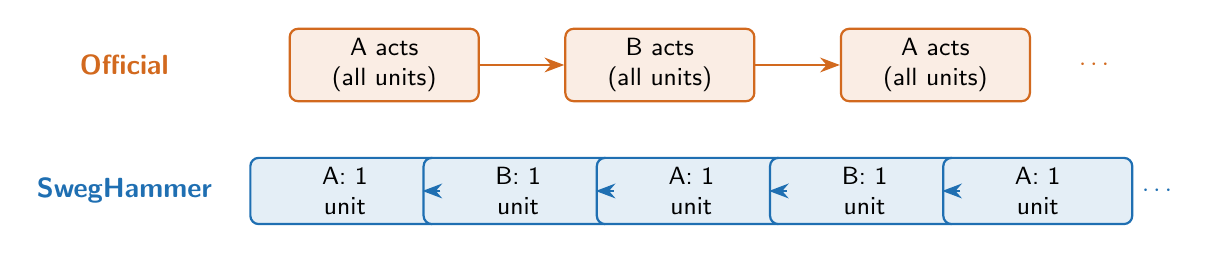
\begin{tikzpicture}[
    >={Stealth[length=2.5mm]},
    every node/.style={font=\sffamily\small},
    phase/.style={rectangle, rounded corners=3pt, draw=#1, thick,
                  fill=#1!12, minimum width=24mm, minimum height=8mm,
                  align=center},
  ]
  % IGOUGO
  \node[font=\sffamily\bfseries, text=realorange] at (-1.8, 0) {Official};
  \node[phase=realorange] (a1) at (1.5, 0) {A acts\\(all units)};
  \node[phase=realorange] (b1) at (5.0, 0) {B acts\\(all units)};
  \node[phase=realorange] (a2) at (8.5, 0) {A acts\\(all units)};
  \draw[->, thick, realorange] (a1) -- (b1);
  \draw[->, thick, realorange] (b1) -- (a2);
  \node[right, text=realorange] at (10.2, 0) {$\cdots$};

  % Alternating
  \node[font=\sffamily\bfseries, text=simblue] at (-1.8, -1.6) {SwegHammer};
  \node[phase=simblue] (sa1) at (1.0, -1.6) {A: 1\\unit};
  \node[phase=simblue] (sb1) at (3.2, -1.6) {B: 1\\unit};
  \node[phase=simblue] (sa2) at (5.4, -1.6) {A: 1\\unit};
  \node[phase=simblue] (sb2) at (7.6, -1.6) {B: 1\\unit};
  \node[phase=simblue] (sa3) at (9.8, -1.6) {A: 1\\unit};
  \draw[->, thick, simblue] (sa1) -- (sb1);
  \draw[->, thick, simblue] (sb1) -- (sa2);
  \draw[->, thick, simblue] (sa2) -- (sb2);
  \draw[->, thick, simblue] (sb2) -- (sa3);
  \node[right, text=simblue] at (11.0, -1.6) {$\cdots$};
\end{tikzpicture}
\end{center}

% ── Section 5: The two-stage pipeline ──────────────────────────────────
\section{The two-stage pipeline}

SwegHammer's work is split into two sequential stages:

\textbf{Stage~1 --- Make the simulator play like reality.} Run the
simulator, compare per-faction win rates against real tournament data (a
10,000-game aggregate from the Warp Friends community), and tweak the
simulator's rules until the simulated results match the real-world results.
The target is a mean absolute error of 2.0 percentage points or less per
faction. This stage is about \textit{simulator fidelity}: if the sim does
not play like the real game, any prices it produces are meaningless.

\textbf{Stage~2 --- Fit the points equation.} Once the simulator is
faithful, freeze its rules and fit one master equation that maps every
unit's stats to a points cost, plus small per-unit corrections for edge
cases. Run the now-trustworthy simulator with equation-priced units, measure
the win-rate spread, adjust the equation's coefficients, and repeat until
every unit hovers near 50\% in equal-points fights. The output is a single
formula that prices any unit from its stat line --- not a hand-tuned table,
but a principled, reproducible result.

% ── Section 6: What's next ─────────────────────────────────────────────
\section{Current status and what comes next}

Stage~1 is in active development. The simulator's mean absolute error
against tournament data currently sits at around 7~percentage points ---
meaningful progress, but still above the 2-point target. Work is focused on
improving the fidelity of faction-specific rules, terrain interactions, and
the strategy layer that governs how simulated units choose their actions.

Stage~2 tooling is built and running in parallel, but its outputs are
provisional until Stage~1 converges. Once the simulator plays like the real
game, the points equation will be re-fitted against the faithful simulation,
producing the final balanced points costs.

The long-term vision is a community tool where players can look up
simulation-derived points for any unit, explore what-if scenarios (``what if
this unit had one more wound?''), and play games with SwegHammer-balanced
army lists.

\vfill

\begin{center}
  \small\color{greytext}
  SwegHammer is an open-source project.\\
  Repository: \url{https://github.com/eddiehandford/sweghammer}
\end{center}

\newpage

% ── Example Datasheets ─────────────────────────────────────────────────
\section{Example datasheets}
\label{sec:datasheets}

The two datasheets below illustrate the extremes of the game's unit
spectrum. The \textit{Intercessor Squad} is a bread-and-butter infantry
squad --- cheap, numerous, and straightforward. The \textit{Knight Crusader}
is a towering war machine that costs almost five times as much and carries
an arsenal of heavy weapons. The points system must make a game between
five Intercessor squads and one Knight Crusader feel fair.

Full datasheets with special abilities and stratagems are available on
Wahapedia (links below each table).

\vspace{4mm}

% ── Intercessor Squad ─────────────────────────────────────────────────
\subsection{Intercessor Squad \normalfont\small(Space Marines)}

\begin{center}
\renewcommand{\arraystretch}{1.2}
\begin{tabular}{cccccc}
  \toprule
  \textbf{M} & \textbf{T} & \textbf{Sv} & \textbf{W} & \textbf{Ld} & \textbf{OC} \\
  \midrule
  6\texttt{"} & 4 & 3+ & 2 & 6+ & 2 \\
  \bottomrule
\end{tabular}
\end{center}

\vspace{2mm}

\textbf{Ranged weapons}

\begin{center}
\renewcommand{\arraystretch}{1.2}
\begin{tabular}{l c c c c c c l}
  \toprule
  \textbf{Weapon} & \textbf{Range} & \textbf{A} & \textbf{BS} & \textbf{S} & \textbf{AP} & \textbf{D} & \textbf{Keywords} \\
  \midrule
  Bolt rifle & 24\texttt{"} & 2 & 3+ & 4 & $-1$ & 1 & Assault, Heavy \\
  Bolt pistol & 12\texttt{"} & 1 & 3+ & 4 & 0 & 1 & Pistol \\
  Astartes grenade launcher (krak) & 18\texttt{"} & 1 & 3+ & 9 & $-2$ & D3 & --- \\
  \bottomrule
\end{tabular}
\end{center}

\vspace{2mm}

\textbf{Melee weapons}

\begin{center}
\renewcommand{\arraystretch}{1.2}
\begin{tabular}{l c c c c c}
  \toprule
  \textbf{Weapon} & \textbf{A} & \textbf{WS} & \textbf{S} & \textbf{AP} & \textbf{D} \\
  \midrule
  Close combat weapon & 3 & 3+ & 4 & 0 & 1 \\
  Power weapon (Sergeant) & 4 & 3+ & 5 & $-2$ & 1 \\
  Power fist (Sergeant) & 3 & 3+ & 8 & $-2$ & 2 \\
  \bottomrule
\end{tabular}
\end{center}

\vspace{2mm}

\begin{tabular}{@{}ll@{}}
  \textbf{Unit size:} & 5--10 models \\
  \textbf{Points:} & 80 (Games Workshop) \\
  \textbf{Keywords:} & Infantry, Battleline \\
\end{tabular}

\vspace{1mm}
{\small\color{greytext}
Full datasheet: \url{https://wahapedia.ru/wh40k10ed/factions/space-marines/Intercessor-Squad}}

\vspace{8mm}

% ── Knight Crusader ───────────────────────────────────────────────────
\subsection{Knight Crusader \normalfont\small(Imperial Knights)}

\begin{center}
\renewcommand{\arraystretch}{1.2}
\begin{tabular}{cccccc}
  \toprule
  \textbf{M} & \textbf{T} & \textbf{Sv} & \textbf{W} & \textbf{Ld} & \textbf{OC} \\
  \midrule
  10\texttt{"} & 12 & 3+ & 22 & 6+ & 10 \\
  \bottomrule
\end{tabular}
\end{center}

\vspace{1mm}
\textbf{Invulnerable save:} 5+ (against ranged attacks; 5+ in melee via Ion Shield)

\vspace{2mm}

\textbf{Ranged weapons}

\begin{center}
\renewcommand{\arraystretch}{1.2}
\begin{tabular}{l c c c c c c l}
  \toprule
  \textbf{Weapon} & \textbf{Range} & \textbf{A} & \textbf{BS} & \textbf{S} & \textbf{AP} & \textbf{D} & \textbf{Keywords} \\
  \midrule
  Avenger gatling cannon & 36\texttt{"} & 18 & 3+ & 6 & $-2$ & 2 & --- \\
  Thermal cannon & 24\texttt{"} & 2D3 & 3+ & 12 & $-4$ & D6 & Blast, Melta 2 \\
  Rapid-fire battle cannon & 72\texttt{"} & 2D6+6 & 3+ & 10 & $-1$ & 3 & Blast \\
  Ironstorm missile pod & 48\texttt{"} & D6+1 & 3+ & 5 & 0 & 1 & Blast, Indirect Fire \\
  Stormspear rocket pod & 48\texttt{"} & 3 & 3+ & 8 & $-2$ & D6 & --- \\
  Meltagun & 12\texttt{"} & 1 & 3+ & 9 & $-4$ & D6 & Melta 2 \\
  \bottomrule
\end{tabular}
\end{center}

\vspace{2mm}

\textbf{Melee weapons}

\begin{center}
\renewcommand{\arraystretch}{1.2}
\begin{tabular}{l c c c c c}
  \toprule
  \textbf{Weapon} & \textbf{A} & \textbf{WS} & \textbf{S} & \textbf{AP} & \textbf{D} \\
  \midrule
  Titanic feet & 4 & 4+ & 8 & $-1$ & 2 \\
  \bottomrule
\end{tabular}
\end{center}

\vspace{2mm}

\begin{tabular}{@{}ll@{}}
  \textbf{Unit size:} & 1 model \\
  \textbf{Points:} & 385 (Games Workshop) \\
  \textbf{Keywords:} & Vehicle, Walker, Titanic, Towering, Character \\
  \textbf{Deadly Demise:} & D6 (when destroyed, nearby units suffer D6 mortal wounds) \\
\end{tabular}

\vspace{1mm}

\textbf{Damaged profile:} When this model has 1--7 wounds remaining, subtract 1
from its hit rolls (both ranged and melee), and halve its Move characteristic.

\vspace{1mm}
{\small\color{greytext}
Full datasheet: \url{https://wahapedia.ru/wh40k10ed/factions/imperial-knights/Knight-Crusader}}
\label{sec:datasheets-end}

\end{document}
